\section{Single Layer Perceptrons}
\label{sec:slp}

\begin{frame}
  \begin{center}
    \Huge{\textcolor{red}{Softmax Regression}}
  \end{center}
\end{frame}

\subsection{Softmax}

\begin{frame}[fragile]{符号}
 \begin{itemize}
   \item \textcolor{red}{Training Set}: $ S = \{ ({x^{(i)}},{y^{(i)}});i = 1,2,...,m\} $
   \item \textcolor{red}{Training Example($i_{th}$)}: $ ({x^{(i)}},{y^{(i)}}) $
   \item \textcolor{red}{Input Variable}: $ x = ({x_1},{x_2},...,{x_n})^{T}  \in {\mathbb{R}^n} $
   \item \textcolor{red}{Target Variable}: $ y = ({y_1},{y_2},...,{y_k})^{T} \in {\mathbb{R}^k} $
   \item \textcolor{red}{Weights}: $ W \in {\mathbb{R}^{n \times k}} $   
   \item \textcolor{red}{Bias}: $ b \in {\mathbb{R}^k} $   
   \item \textcolor{red}{Activation}: $ 
softmax {(z_i)} = \tfrac{{{e^{{z_i}}}}}{{\sum\limits_{j = 1}^k {{e^{{z_j}}}} }}  \quad i = 1,2,...,k
$   
 \end{itemize}
\end{frame}


\begin{frame}{模型}
\[\begin{gathered}
  y = softmax ({W^T}x + b) \hfill \\
  x = {({x_1},{x_2},...,{x_n})^T} \in {\mathbb{R}^n} \hfill \\
  y = {({y_1},{y_2},...,{y_k})^T} \in {\mathbb{R}^k} \hfill \\
  W \in {\mathbb{R}^{n \times k}} \hfill \\
  b \in {\mathbb{R}^k} \hfill \\ 
\end{gathered} \]
\end{frame}

\begin{frame}{详解}
\begin{block}{模型}
\[\begin{aligned}
  softmax (z) =  & {({\phi _1},{\phi _2},...,{\phi _k})^T} \\ 
   =  & \tfrac{1}{{\sum\limits_{j = 1}^k {{e^{{z_j}}}} }}{\left( {{e^{{z_1}}},{e^{{z_2}}},...,{e^{{z_k}}}} \right)^T} \\ 
\end{aligned} \]
\end{block}

\begin{block}{解释}
\[\begin{gathered}
  z = {W^T}x + b \in {\mathbb{R}^k} \hfill \\
  \sum\limits_{i = 1}^k {{\phi _j}}  = 1 \hfill \\
  {\phi _i} = \tfrac{{{e^{{z_i}}}}}{{\sum\limits_{j = 1}^k {{e^{{z_j}}}} }} \hfill \\ 
\end{gathered} \]
\end{block}
\end{frame}

\begin{frame}{损失函数}
\[E =  - \sum\limits_{i = 1}^m {{y^{(i)}}\log } \left( {{{\widehat y}^{(i)}}} \right)\]
\end{frame}

\subsection{Mnist}

\begin{frame}{图片:$ 28x28 = 784 $}
  \begin{figure}
    \centering
    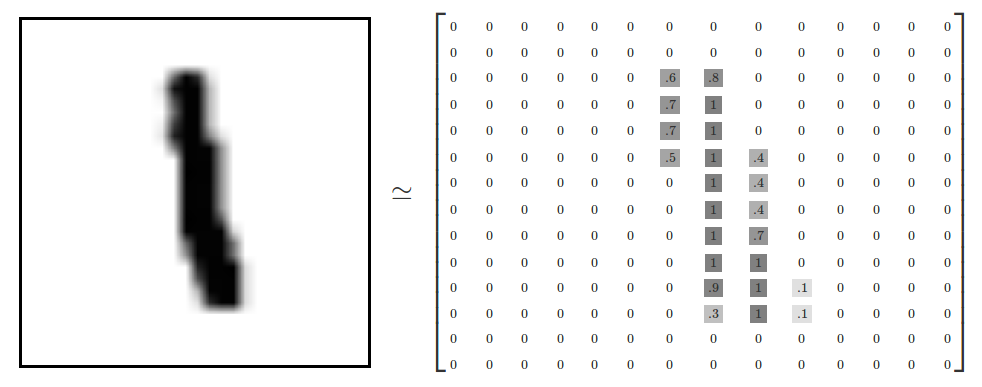
\includegraphics[width=0.8\textwidth]{mnist-matrix.png}
  \end{figure}
\end{frame}

\begin{frame}{训练数据集输入:$ [60000, 784] $}
  \begin{figure}
    \centering
    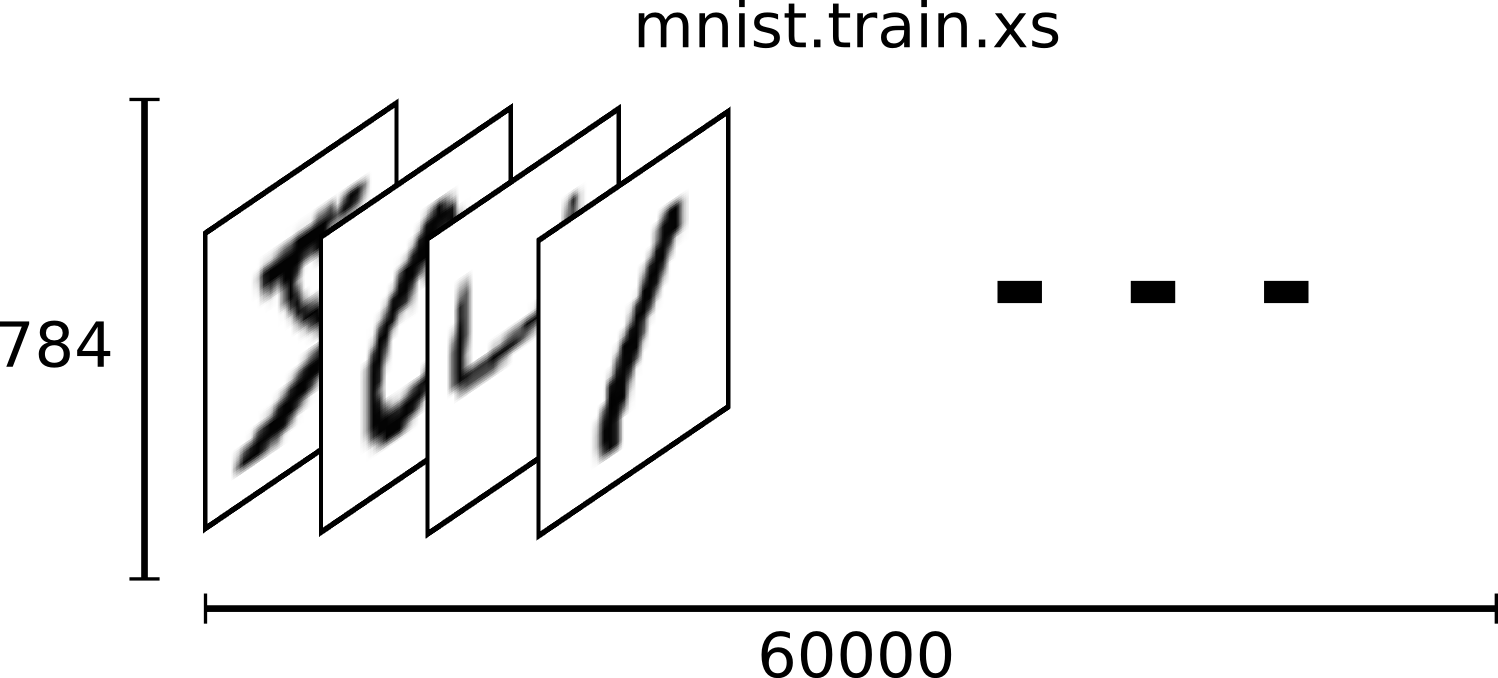
\includegraphics[width=0.8\textwidth]{mnist-train-xs.png}
  \end{figure}
\end{frame}

\begin{frame}{训练数据集输出:$ [60000, 10] $}
  \begin{figure}
    \centering
    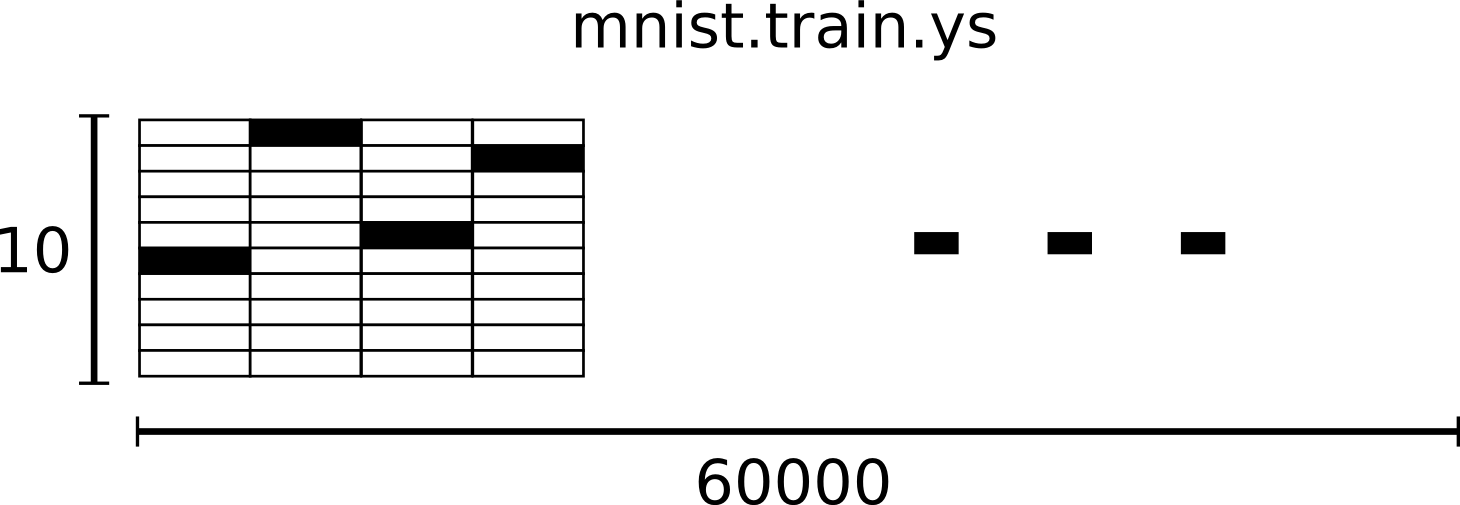
\includegraphics[width=0.8\textwidth]{mnist-train-ys.png}
  \end{figure}
\end{frame}

\begin{frame}[fragile]{导入TensorFlow}
\begin{python}
import tensorflow as tf
\end{python}
\end{frame}

\begin{frame}[fragile]{占位符}
\begin{python}
x  = tf.placeholder("float", [None, 784])  
y_ = tf.placeholder("float", [None,10])
\end{python}

\begin{itemize}
  \item \code{placeholder}定义了一个占位\code{op}
  \item \code{None}表示任意的样本数目
  \item 待\code{session.run}时提供(feed)
\end{itemize}
\end{frame}

\begin{frame}[fragile]{变量}
\begin{python}
W = tf.Variable(tf.zeros([784,10]))
b = tf.Variable(tf.zeros([10]))

init = tf.initialize_all_variables()
\end{python}

\begin{itemize}
  \item \code{Variable}代表了一个可修改的\code{Tensor}
  \item 此处初始化为\code{0},但并未真正执行
  \item 初始化由\code{init}的\code{op}完成,并延迟至\code{session.run}执行
\end{itemize}

\end{frame}

\begin{frame}[fragile]{模型}
\begin{python}
y = tf.nn.softmax(tf.matmul(x,W) + b)
\end{python}

\[{y_{60000 \times 10}} = softmax ({x_{60000 \times 784}}{W_{784 \times 10}} + {b_{60000 \times 10}})\]

\end{frame}

\begin{frame}[fragile]{优化算法:Adam}
\begin{python}
cross_entropy = -tf.reduce_sum(y_*tf.log(y))
train_step = tf.train.AdamOptimizer(1e−4).minimize(cross_entropy)
\end{python}

\begin{block}{损失函数}
\[\begin{aligned}
  E =  & - \sum\limits_{i = 1}^m {{y^{(i)}}\log } \left( {{{\widehat y}^{(i)}}} \right) \\ 
  {\widehat y^{(i)}} =  & \; softmax ({W^T}{x^{(i)}} + b) \\ 
\end{aligned} \]
\end{block}
\end{frame}

\begin{frame}[fragile]{执行计算图}
\begin{python}
sess = tf.Session()
sess.run(init)

for i in range(1000):
  batch_xs, batch_ys = mnist.train.next_batch(100)
  sess.run(train_step, feed_dict={x: batch_xs, y_: batch_ys})
\end{python}

\begin{itemize}
  \item MiniBatch算法:\code{epoch = 1000, batch\_size = 100}
  \item 首先执行\code{op(init)},完成变量(Varibales)的初始化
  \item 执行\code{op(train\_step)},联带执行\code{ops(cross\_entropy, x, y\_)}
  \item 并feed相应的数据给\code{ops(x, y\_)}
\end{itemize}

\end{frame}